\documentclass[answers]{exam}
\usepackage{graphicx}
\usepackage{wrapfig}
\usepackage[utf8]{inputenc}

\pagestyle{headandfoot}
\lhead{PSYCH 260/BBH 203}
\chead{}
\rhead{Quiz 1}

\title{PSYCH 260 Quiz 1}
\author{}
\date{September 14, 2015}

\begin{document}

\maketitle

\section{Main - 10 pts}

\begin{questions}

\begin{figure}[h]
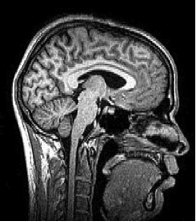
\includegraphics[width=0.25\textwidth]{images/brain.jpg}
\centering
\end{figure}

\question The image illustrates what type of slice?
\begin{choices}
 \correctchoice Sagittal
 \choice Horizontal
 \choice Coronal
 \choice Axial
\end{choices}

\question All of the following structures can be seen in the figure EXCEPT
\begin{choices}
\choice Cerebellum
\choice Corpus callosum
\correctchoice Lateral ventricles
\choice Cerebral cortex
\end{choices}

\question The figure illustrates which imaging method?
\begin{choices}
\choice CT
\choice PET
\choice Magnetoencephalography (MEG)
\correctchoice MRI
\end{choices}

\newpage

\question Descartes thought that this structure was the place where the soul influenced the human body's voluntary movements.
\begin{choices}
\choice The pons
\choice The pituitary gland
\correctchoice The pineal gland
\choice The reflexive complex
\end{choices}

\question The tongue is \fillin with respect to the nose.
\begin{choices}
\correctchoice Ventral
\choice Superior
\choice Dorsal
\choice Medial
\end{choices}

\question Auditory information enters the CNS via the 8th (VIII) cranial nerve and projects through this sound-responsive nucleus of the midbrain tectum.
\begin{choices}
\choice lateral geniculate nucleus
\choice striatum
\choice substantia nigra
\correctchoice inferior colliculus
\end{choices}

\question Neural degeneration in this structure is associated with Parkinson’s Disease.
\begin{choices}
\choice hypothalamus
\correctchoice substantia nigra
\choice insula
\choice amygdala
\end{choices}

\question Electroencephalography (EEG) has \fillin temporal resolution than functional MRI, \\
but \fillin spatial resolution.
\begin{choices}
\choice better; similar
\correctchoice better; worse
\choice worse; better
\choice worse; similar
\end{choices}

\question Which of these landmarks separates the frontal from the parietal lobe?
\begin{choices}
\choice Lateral fissure
\choice Longitudinal fissure
\choice Anterior cingulate gyrus
\correctchoice Central sulcus
\end{choices}

\question Gray matter is mainly composed of:
\begin{choices}
    \choice Axons
    \correctchoice Cell bodies
    \choice Myelin
    \choice None of the above
\end{choices}

\section{Bonus}
\question Which of these is NOT a component of the forebrain?
\begin{choices}
\choice Cerebral cortex
\choice Basal ganglia
\choice Hypothalamus
\correctchoice Medulla
\end{choices}	

\end{questions}

\end{document}